\documentclass[11pt]{book}

\usepackage{amsmath}
\usepackage{amssymb}
\usepackage{graphicx}
\graphicspath{{.} {/home/gantry/Projects/gantryderivations} }
\DeclareGraphicsExtensions{.pdf,.png,.jpg}


\title{\textbf{Gantry's\\Mathematical Proofs,\\Derivations, Conjectures\\and Explanations}}
\author{Gantry York}
\date{May 20, 2013}

\begin{document}

\maketitle

\tableofcontents 


\chapter*{Overview}

\section*{Why This Book}
I was not a great math student in high school.  My grades were good, but I was learning how to apply formulas and execute methods.\\
\\
It wasn't until I took calculus at the university that I actually understood where the formulas came from.\\
\\
This was my epiphany.  This is when these symbols and operations started to mean something to me.  I would say it was analagous from going from grammar to literature.  This is when the mathematics started to tell me a story\\
\\
For many students, deriving a formula is not imporant to them since the homework sets are about apply the formula.  But if you want to truly understand a formula, it's boundary conditions, when it does and does not apply, extrapolate it beyond it's context, you must have an appreciation for the derivation.\\
\\


\section*{Terminology}
Many consider a proof and a derivation as essentially the same thing.\\
\\
A proof is when you state: If p, then q\\
\\
Here p is a fundamental statement(s) that are assumed to be true.  If you accept it to be true, it is called an \emph{axiom}.\\
\\
p is refered to as the \emph{hypothesis} or \emph{proposition}, and q is refered to as the \emph{conclusion}.\\
\\
To prove q true, one must start with p and provide a convincing argument that leads to q.\\
\\
If this is done in intermediate parts, these parts are called \emph{lemmas}.\\
\\
So after stating if p, then q, one makes derivative statements of p with the intended purpose of leading to q.  This is the \emph{derivation}.\\
\\
Derivations are also used less formally outside the context of a formal proof.\\
\\
A \emph{conjecture} is an unproven proposition that one can make a compelling but incomplete argument that it is true.  This could be a visual proof; proving it to be true for most cases; an extrapolation of logic; a demonstration of pattern; or other such reasoning.\\
\\
 
\chapter{Geometry}

\section{Sum of Exterior Angles of a Polygon}

The sum of the exterior angles of a polygon is \(360^{\circ}\)
\[Sum_{ext} = 360^{\circ}\]
\\
As long as the polygon has no concavity to its shape.

\subsection{Conjecture}

By definition, all the angles in a circle sum up to be \(360^{\circ}\) \\
\[\sum\limits_{n=1}^{N}{a_n} = 360^{\circ}\] \\

\begin{center}
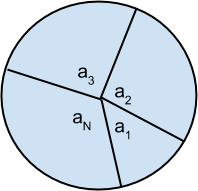
\includegraphics[width=8cm]{polygon_ext_angles_diag1}
\end{center}
The lines can be extended and removed from the center, while still keeping their orientation. \\
\begin{center}
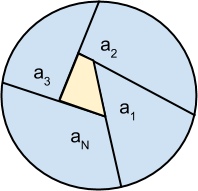
\includegraphics[width=8cm]{polygon_ext_angles_diag2}
\end{center}
The relative angles, \(a_n\), between each line remains the same, and a polygon is formed in the middle.\\
\\
This is only true for polygons that can be created using this method.  A polygon like the one below is impossible to create using this method. \\
\\
\begin{center}
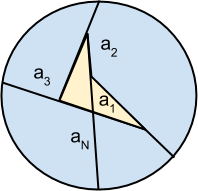
\includegraphics[width=8cm]{polygon_ext_angles_diag3}
\end{center}
Hence, \(Sum_{ext} = 360^{\circ}\) is true only for polygons with no concavity \\
\\

\section{Sum of Interior Angles of a Polygon}
The sum of the interior angles of a polygon is
\[Sum_{ing} = (N-2)180^{\circ}\] \\
where N is the number of sides of the polygon\\
\\
As long as the polygon has no concavity to its shape.\\
\\
\subsection{Derivation}

The sum of all the exterior angles is 
\[\sum\limits_{n=1}^{N}{a_n} = 360^{\circ}\] \\
\\
Exterior and interior angles are the compliments of each other.  So if \(a_n\) is the exterior angle, then \(180-a_n\) is the interior angle and \\

\begin{align*}
Sum_{int} &= \sum\limits_{i=1}^N{180^{\circ}-a_n}\\
&= 180^{\circ}\sum\limits_{i=1}^N{1}-\sum\limits_{i=1}^N{a_n}\\
&= 180^{\circ}\sum\limits_{i=1}^N{1}-360^{\circ}\\
&= 180^{\circ}N-360^{\circ}\\
Sum_{int} &= (N-2)180^{\circ}
\end{align*}
\\

\section{Area of a Rectangle}

\section{Area of a Triangle}

\subsection{Derivation: $\frac{1}{2}bh$}

\subsection{Derivation: Heron's formula}

\section{Area of a Circle}

The area of a circle is most commonly stated as

\[A = \pi r^2\]
\\
where \(r\) is the radius of the circle

\subsection{Derivation: Cartesian coordinates}

\subsection{Derivation: Polar coordinates}
The easiest derivation of the area of a circle is to simply use polar coordinates where the differential volume is 
\[dv = rd\theta dr\]

\begin{align*}
A =& \oint dv \\
A =& \int\limits_{0}^{2\pi}\int\limits_{0}^{r} rd\theta dr \\
A =& \bigg[ \theta \bigg|_{0}^{2\pi}\bigg[ \frac{1}{2}r^2 \bigg|_{0}^{r} \\
A =& [2\pi - 0]\frac{1}{2}[r-0] \\
A =& \pi r^2
\end{align*}
\\
\subsection{Conjecture: No Calculus}

Inscribe an N-sided polygon in a circle or radius \(R\).  Each interior angle will be \(\theta =\frac{2\pi}{N}\).  The polygon will be made up of \(N\) triangles.  Each of these triangles will have an area of
\[A_{triangle} = \frac{bh}{2} = \frac{R\cos(\frac{\theta}{2})2R\sin(\frac{\theta}{2})}{2}\]
And the area of the polygon will be
\begin{align*}
A_{poly} =& NR\cos(\frac{\theta}{2})R\sin(\frac{\theta}{2})\\
A_{poly} =& R^2N\cos(\frac{\pi}{N})\sin(\frac{\pi}{N})\\
\end{align*}
What happens when you increase \(N\) larger and larger and large?  What happens when \(N\) approaches infinity\\
\\
We can use the approximations\\
\(\sin(\alpha) \approx \alpha\), for really small \(\alpha\)\\
and of course\\
\(\\cos(0) = 1\)\\
\\
So
\begin{align*}
A_{poly} =& A_{circ} = R^2\cos(\frac{\pi}{N})N\sin(\frac{\pi}{N})\\
A_{poly} =& A_{circ} = R^2(1))(N\frac{\pi}{N}))\\
A_{circ} =& \pi R^2
\end{align*}

\section{Volume of a Sphere}

\section{Surface Area of a Cone}

\chapter{Trigonometry}

\section{Pythagorean Theorem}
The Pathagrean Theorem is most commonly stated as
\[a^2 + b^2 = c^2\]
\\
Where a and b refer to the legs of a right triangle and c refers to the hypotenuse.\\
\\
\subsection{Derivation}
A square can be constructed of 4 right triangles as shown below.\\
\begin{center}
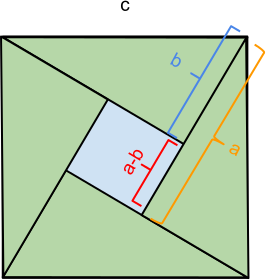
\includegraphics[width=8cm]{pythagorus_diag1}
\end{center}
The area of the square, \(c^2\), is equal to the area of the 4 right triangles plus the area of the inner square.\\

\begin{align*}
c^2 =& 4\frac{ab}{2} + (a-b)^2\\
c^2 =& 2ab + a^2 -2ab + b^2 \\
c^2 =& a^2 + b^2
\end{align*}

\section{Sum and Difference of Sine}

\section{Sum and Difference of Cosine}

\section{Double Angle Identity for Sine}
The Double Angle Identity for sine is most commonly stated as
\[\sin{(2u)} = 2\sin{(u)}cos{(u)}\]

\subsection{Derivation}

\begin{center}
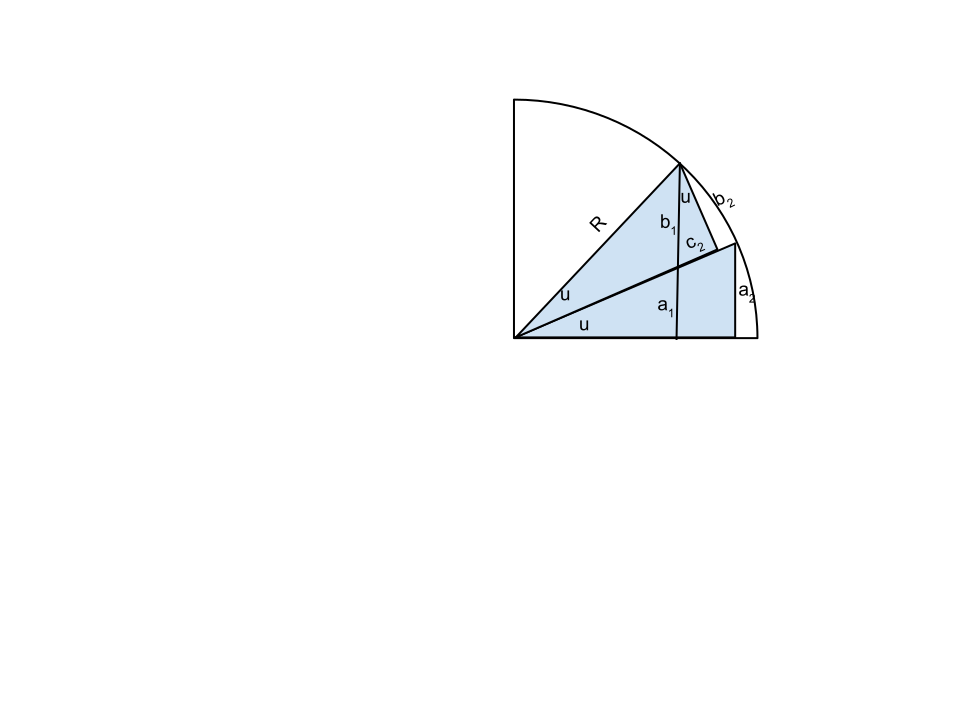
\includegraphics[width=8cm]{Sine_double_angle}
\end{center}

With respect to the diagram above
\[R\sin{(2u)} = a_1 + b_1\]
Find \(a_1 \text{ and } b_1\)\\
\\
For \(a_1\) \\
\begin{align*}
a_1 &= c_2\sin{(u)} \\
c_1 + c_2 &= R\cos{(u)} \\
c_1 &= b_1\sin{(u)} \\
c_2 &=  R\cos{(u)} - b_1\sin{(u)} \\ 
a_1 &= (R\cos{(u)} - b_1\sin{(u)})\sin{(2u)}
\end{align*}
\\
For \(b_1\) \\
\begin{align*}
b_2 &= a_2 \\
b_1\cos{(u)} &= R\sin{(u)} \\
b_1 &= R\tan{(u)}
\end{align*}
\\
So
\begin{align*}
R\sin{(2u)} &= a_1 + b_1 \\
R\sin{(2u)} &= (R\cos{(u)} - b_1\sin{(u)})\sin{(u)} + b_1 \\
R\sin{(2u)} &= R\cos{(u)}\sin{(u)} -b_1\sin^2{(u)} +b_1 \\
R\sin{(2u)} &= R\cos{(u)}\sin{(u)} + b_1(1 -\sin^2{(u)})\\
R\sin{(2u)} &= R\cos{(u)}\sin{(u)} + b_1\cos^2{(u)} \\
R\sin{(2u)} &= R\cos{(u)}\sin{(u)} + R\tan{(u)}\cos^2{(u)} \\
sin{(2u)} &= \cos{(u)}\sin{(u)} + \sin{(u)}\cos{(u)} \\
sin{(2u)} &= 2\sin{(u)}\cos{(u)} 
\end{align*}
\\
Thus
\[sin{(2u)} = 2\sin{(u)}\cos{(u)} \]

\section{Double Angle Identity for Cosine}

\chapter{Algebra}

\section{$(a+b)^2$}
The square of the sum of two numbers is
\[(a+b)^2 = a^2 +2ab +b^2\]

\subsection{Derivation}
\begin{center}
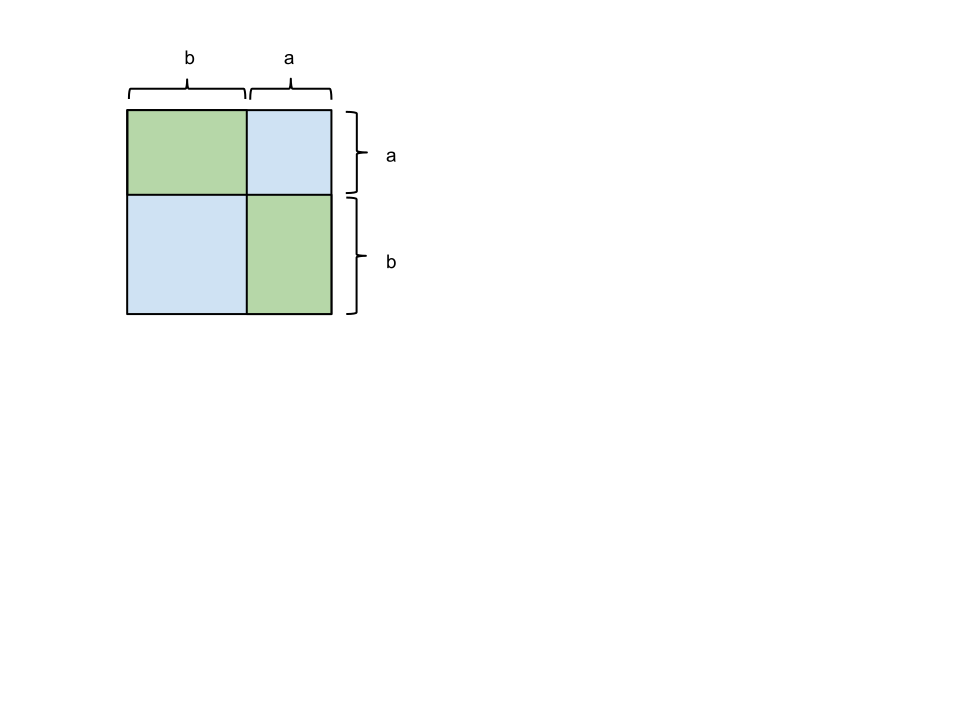
\includegraphics[width=8cm]{binomial_square_diag1}
\end{center}
The area of the square above is \((a+b)^2\) \\
It is also the sum of the 4 individual squares\\
\begin{align*}
(a+b)^2 &= aa + ab + ab + bb\\
(a+b)^2 &= a^2 +2ab + b^2
\end{align*}

\section{$(a+b)^3$}

\section{Binomial Theorem}

\section{Quadratic Equation}
The Quadratic Equation is most commonly stated as \\\\
Given the second order polynominal, \(ax^2 + bx + c = 0\)\\
the roots of equation are, \(x = \dfrac{-b \pm \sqrt{b^2 -4ac}}{2a}\) \\
but \(a \ne 0\)

\subsection{Derivation}

Let's rewrite \(ax^2+bx+c = 0 \) using the technique of Completing the Square \\
\begin{align*}
x^2 + \frac{b}{a} + \frac{c}{a} &= 0 \\
x^2 + \frac{b}{a} &= -\frac{c}{a} \\
x^2 + \frac{b}{a} + \left(\frac{1}{2}\frac{b}{a}\right)^2 &= -\frac{c}{a} + \left(\frac{1}{2}\frac{b}{a}\right)^2 \\
\left(x + \frac{b}{2a}\right)^2 &= -\frac{c}{a} + \frac{b^2}{4a^2} \\
\left(x + \frac{b}{2a}\right)^2 &= \frac{-4ac +b^2}{4a^2} \\
\end{align*}
Now just solve for x
\begin{align*}
x + \frac{b}{2a} &= \sqrt{\frac{b^2 -4ac}{4a^2}} \\
x  &= -\frac{b}{2a} \pm \sqrt{\frac{b^2 -4ac}{4a^2}}  \\
x &= \dfrac{-b \pm \sqrt{b^2 -4ac}}{2a}
\end{align*}

\chapter{Linear Algebra}

\section{Rotational Matrix for $\mathbb{R}^2$}
The Rotational Matrix for rotating a coordinate system in 2 dimensions is commonly stated as
\[
R(\theta) = \left[ \begin{matrix}
\cos(\theta) & -\sin(\theta) \\
sin(\theta) &  \cos(\theta) 
\end{matrix}\right]
\]
Where it is applied to a Cartesian cordinate system as
\[
\left[ \begin{matrix}
\cos(\theta) & -\sin(\theta) \\
\sin(\theta) &  \cos(\theta) 
\end{matrix}\right] 
\left[ \begin{matrix}
x' \\
y'
\end{matrix} \right] =
\left[ \begin{matrix}
x \\
y
\end{matrix} \right]
\]
where x' and y' are the rotated coordinates.

\subsection{Derivation}
A positional vector denotes a point (x,y) in the Cartesian Coordinate System.  This positional point has an angle of \(\theta\) and a magnitude of \(\sqrt{x^2 + y^2}\) \\
\\
\begin{center}
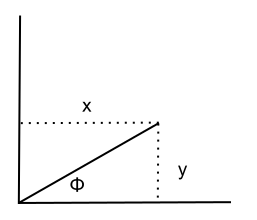
\includegraphics[width=8cm]{rotational_matrix_diag1}
\end{center}

Now rotate the entire coordinate system by an angle \(\theta\)\\
\begin{center}
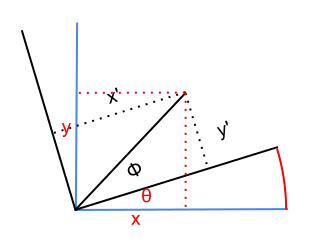
\includegraphics[width=8cm]{rotational_matrix_diag2}
\end{center}

\begin{align*}
x &= \sqrt{(x')^2 + (y')^2}\cos(\phi + \theta) \\
y &= \sqrt{(x')^2 + (y')^2}\sin(\phi + \theta)\\
\\
x &= \sqrt{(x')^2 + (y')^2}(\cos(\phi)\cos(\theta) - \sin(\phi)\sin(\theta) ) \\
y &= \sqrt{(x')^2 + (y')^2}(\sin(\phi)\cos(\theta) + cos(\phi)sin(\theta) )\\
\\
x &= x'\frac{\sqrt{(x')^2 + (y')^2}}{x'}(\cos(\phi)\cos(\theta) - \sin(\phi)\sin(\theta) ) \\
y &= y'\frac{\sqrt{(x')^2 + (y')^2}}{y'}(\sin(\phi)\cos(\theta) + \cos(\phi)\sin(\theta) )\\
\\
x &= x'\frac{1}{\cos(\phi)}(\cos(\phi)\cos(\theta) - \sin(\phi)\sin(\theta) ) \\
y &= y'\frac{1}{\sin(\phi)}(\sin(\phi)\cos(\theta) + \cos(\phi)\sin(\theta) )\\
\\
x &= x'(\cos(\theta) - \tan(\phi)\sin(\theta) ) \\
y &= y'(\cos(\theta) + \cot(\phi)sin(\theta) ) \\
\\
x &= x'(\cos(\theta) - \frac{y'}{x'}\sin(\theta) ) \\
y &= y'(\cos(\theta) + \frac{x'}{y'}\sin(\theta) ) \\
\\
x &= x'\cos(\theta) - y'\sin(\theta) \\
y &= y'\cos(\theta) + x'\sin(\theta)  \\
\\
\left[
\begin{matrix}
x\\
y
\end{matrix}
\right] &=
\left[ \begin{matrix}
\cos(\theta) & -\sin(\theta) \\
\sin(\theta) &  \cos(\theta) 
\end{matrix}\right] 
\left[ \begin{matrix}
x' \\
y'
\end{matrix} \right]
\end{align*}

\section{Rotational Matrix for $\mathbb{R}^3$}
The Rotational Matrices in 3 dimensions can be stated as
\[
R_z(\theta) = \left[ \begin{matrix}
\cos(\theta) & -\sin(\theta) & 0\\
\sin(\theta) &  \cos(\theta) & 0\\
0 & 0 & 1 
\end{matrix}\right]
\]
For a rotation about the z-axis\\
\[
R_y(\theta) = \left[ \begin{matrix}
\cos(\theta) &  0 &-\sin(\theta) \\
0 & 1 & 0 \\
\sin(\theta) &  0 &\cos(\theta)\\
\end{matrix}\right]
\]
For a rotation about the y-axis
\[
R_x(\theta) = \left[ \begin{matrix}
1 & 0 & 0\\
0 & \cos(\theta) & -\sin(\theta) \\
0 & \sin(\theta) &  \cos(\theta) \\
\end{matrix}\right]
\]
For a rotation about the x-axis
\\
\subsection{Explanation}
It's almost obvious that from \\
\[
\left[ \begin{matrix}
\cos(\theta) & -\sin(\theta) \\
\sin(\theta) &  \cos(\theta) 
\end{matrix}\right] 
\left[ \begin{matrix}
x' \\
y'
\end{matrix} \right] =
\left[ \begin{matrix}
x \\
y
\end{matrix} \right]
\]
We can extend it to\\
\[
\left[ \begin{matrix}
\cos(\theta) & -\sin(\theta) & 0\\
\sin(\theta) &  \cos(\theta) & 0\\
0 & 0 & 1
\end{matrix}\right] 
\left[ \begin{matrix}
x' \\
y' \\
z'
\end{matrix} \right] =
\left[ \begin{matrix}
x \\
y \\
z
\end{matrix} \right]
\]
And this could be exteneded beyond 3 dimensions.\\
\\
It is important to note that the order of these rotations is important
\[R_zR_yR_xX \ne R_xR_yR_zX\]
\\
To demonstrate this take a Rubik's Cube and orient it with the white side facing up, blue facing front, orange facing right (yellow down, red left, green back).  This is your starting position. \\
\\
Now rotate:\\
clockwise about the front, clockwise about the top, clockwise about the right.\\
\\
This is not the result if you do the reverse order:\\
clockwise about the right, clockwise about the top, clockwise about the front\\
\\
This is because matrix multiplication is not commutative.

\chapter{Summations}

\section{Sum of a Constant}

\section{Sum of a Finite Geometric Series}
The sum of the Geometric Series is most commonly stated as
\[ \sum_{i=0}^N{a^i} = \frac{1 - a^{N+1}}{1-a} \]

\subsection{Derivation}
\begin{align*}
\sum_{i=0}^N{a^i} &= a^0 + a^1 + a^2 + ... + a^N  \\
a\sum_{i=0}^N{a^i} &= a^1 + a^2 + ... + a^N + a^{N+1}
\end{align*}
Subtract the two equations
\begin{align*}
\sum_{i=0}^N{a^i} - a\sum_{i=0}^N{a^i} &= a^0 - a^{N+1}  \\
(1-a)\sum_{i=0}^N{a^i} &= 1 - a^{N+1} \\
\sum_{i=0}^N{a^i} &= \frac{1 - a^{N+1}}{1-a}
\end{align*}

\section{Sum of an Infinite Geometric Series}
The sum of the Geometric Series is most commonly stated as
\[ \sum_{i=0}^\infty{a^i} = \frac{1}{1-a} \]
if and only if \(a<1\)

\subsection{Derivation}
If we start with the summation of the finite Geometric Series, then take the limiting case where \(N\to \infty\) \\

\begin{align*}
\lim_{N\to \infty} \sum_{i=0}^N{a^i} = \frac{1 - a^{N+1}}{1-a} \\
\sum_{i=0}^\infty{a^i} = \frac{1 - \lim_{N\to \infty}a^{N+1}}{1-a}
\end{align*}
\\
\(\lim_{ N\to \infty}a^{N+1} =0 \) if and only if \(a<1\) \\
\begin{align*}
\sum_{i=0}^\infty{a^i} = \frac{1}{1-a}
\end{align*}
if and only if \(a<1\)


\section{$\sum\limits_{i=0}^N{i}$ : The Arithmatic Series}
The sum of the Arithmatic Series is most commonly stated as
\[\sum_{i=0}^N i= \sum_{i=1}^N i = \frac{N(N+1)}{2} \]

\subsection{Conjecture}
We can visualize adding 1 block to 2 blocks to 3 blocks and continue until we have N blocks.  As you can see, it sort of forms a triangle. \\
\begin{center}
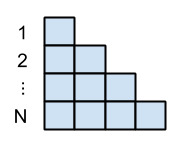
\includegraphics[width=6cm]{sum_i_diag1}
\end{center}
What if we took the same triangle of blocks, flipped it upside down and joined it with the existing triangle?  It would form a rectangle of dimensions N x N+1. \\
\begin{center}
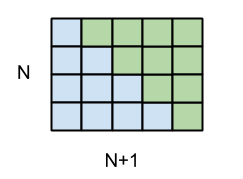
\includegraphics[width=8cm]{sum_i_diag2}
\end{center}
The area of this is \[A_{rectangle} = N(N+1)\] \\
\\
But what we want is the area of the tringle, just half of that \[A_{triangle}=\frac{N(N+1)}{2}\]
And this is \[ \sum_{i=0}^N i= \sum_{i=1}^N i = \frac{N(N+1)}{2}\]


\section{$\sum\limits_{i=0}^N{i^2}$}
The sum of \(i^2\) is most commonly stated as
\[\sum\limits_{i=0}^N{\frac{N(N+1)(2N+1)}{6}}\]

\subsection{Conjecture}
The same technique as used to demonstrate \(\sum\limits_{i=0}^N{i}\) can be used to demonstrate \(\sum\limits_{i=0}^N{i^2}\), except we have to use a 3-dimensional object.\\
\(\sum\limits_{i=0}^N{i^2}\) can be visualized in 3-dimensions as follows
\begin{center}
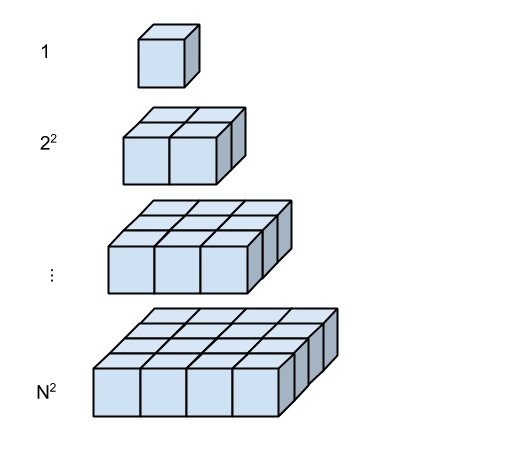
\includegraphics[width=8cm]{sum_i2_diag1}
\end{center}
Then a cube of dimensions N x (N+1) x (N+1) could be made.  See the diagram below\\
\begin{center}
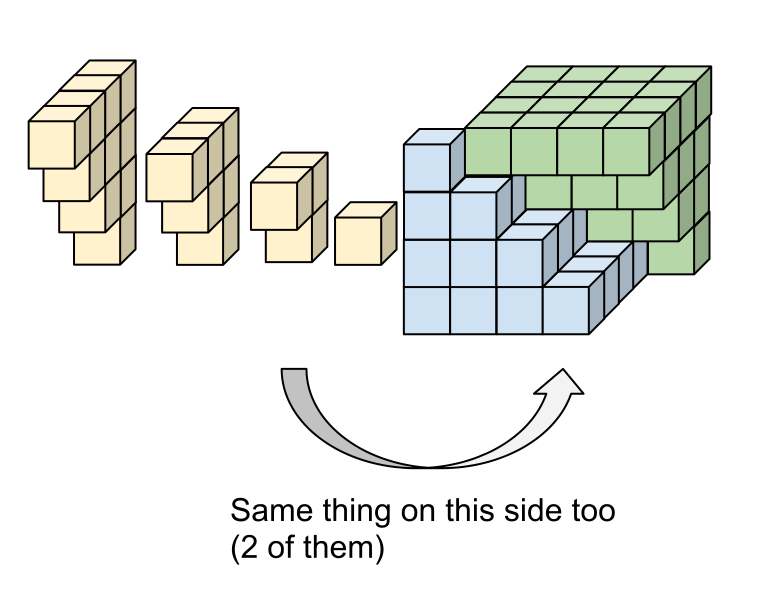
\includegraphics[width=8cm]{sum_i2_diag2}
\end{center}
The blue of the blue cubes is \(\sum\limits_{i=0}^N{i^2}\).  \\
The green of the blue cubes is \(\sum\limits_{i=0}^N{i^2}\).  \\
\\
The yellow cubes are \(\sum\limits_{i=0}^N{i}\), \(\sum\limits_{i=0}^{N-1}{i}\), \(\sum\limits_{i=0}^{N-2}{i}\), ...   \\
Or a more general way to write this would be \(\sum\limits_{i=0}^N{ \sum\limits_{j=0}^i{j}}\) \\
\\
\[ V_{prism} = N(N+1)^2 = 2\bigg(\sum\limits_{i=0}^N{i^2}\bigg) + 2\bigg(\sum\limits_{i=0}^N{ \sum\limits_{j=0}^i{j}} \bigg) \] \\
\begin{align*}
N(N+1)^2 =& 2\bigg(\sum\limits_{i=0}^N{i^2}\bigg) + 2\bigg(\sum\limits_{i=0}^N{ \frac{i(i+1)}{2}} \bigg) \\
N(N+1)^2 =& 2\sum\limits_{i=0}^N{i^2} + \sum\limits_{i=0}^N{ (i^2 + i)} \\
N(N+1)^2 =& 2\sum\limits_{i=0}^N{i^2} + \sum\limits_{i=0}^N{i^2 } + \sum\limits_{i=0}^N{i} \\
N(N+1)^2 =& 3\sum\limits_{i=0}^N{i^2} + \frac{N(N+1)}{2} \\
3\sum\limits_{i=0}^N{i^2} =& N(N+1)^2 - \frac{N(N+1)}{2} \\
3\sum\limits_{i=0}^N{i^2} =& \frac{3N(N+1)^2 - N(N+1)}{2} \\
\sum\limits_{i=0}^N{i^2} =& \frac{2N^3+3N^2+N}{6} \\
\end{align*}
And so
\[\sum\limits_{i=0}^N{i^2} = \frac{N(N+1)(2N+1)}{6}\] \\


\section{$\sum\limits_{i=0}^N{i^3}$ and beyond}
The sum of \(i^3\) is most commonly stated as
\[\sum\limits_{i=0}^N{i^3} = \bigg(\frac{N(N+1)}{2} \bigg)^2 = \bigg[\sum\limits_{i=0}^N{i^2} \bigg]^2\]

\subsection{Derivation}
The sum of \(i\) was derived by visualizing the stacking of 1-dimensional objects into a 2-dimensional shape.  Similarly, the sum of \(i^2\) was derived from stacking 2-dimensional objects into a 3-dimensional object. \\
\\
Unfortunately, our brains are not wired to visualize 4-dimensional objects, so we are left to derive the sum of \(i^3\) this with the abstraction of mathematics. \\
\\
The following is a mathematical technique that will be used to derive the sum of \(i^3\), however, the same technique may be used to the sum of \(i^p\)\\
\\
\(\sum\limits_{i=1}^N{i^4} = 1^4 + 2^4 + ... + N^4 \) \\
and \\
\(\sum\limits_{i=1}^N{(i+1)^4} = 2^4 + ... + N^4 + (N+1)^4\) \\
\\
These two sequences are equal if we take away the first term of the first summation and the last term of the second summation. \\
\begin{align*}
\bigg(\sum\limits_{i=1}^N{i^4} \bigg) - 1^4 = \bigg( \sum\limits_{i=1}^N{(i+1)^4} \bigg) -(N+1)^4 \\
\sum\limits_{i=1}^N{(i+1)^4} = \bigg(\sum\limits_{i=1}^N{i^4} \bigg) + (N+1)^4 - 1^4 \\
\sum\limits_{i=1}^N{(i^4 +4i^3 + 6i^2 + 4i +1)} = \bigg(\sum\limits_{i=1}^N{i^4} \bigg) + (N+1)^4 - 1^4 \\
\sum\limits_{i=1}^N{i^4} + 4\sum\limits_{i=1}^N{i^3} + 6\sum\limits_{i=1}^N{i^2} +4\sum\limits_{i=1}^N{i} + \sum\limits_{i=1}^N{1} = \bigg(\sum\limits_{i=1}^N{i^4} \bigg) + (N+1)^4 - 1^4 \\
4\sum\limits_{i=1}^N{i^3} = (N+1)^4 - 1^4  - 6\sum\limits_{i=1}^N{i^2} - 4\sum\limits_{i=1}^N{i} - \sum\limits_{i=1}^N{1} \\
 4\sum\limits_{i=1}^N{i^3} = (N+1)^4 - 1^4  - 6\bigg(\frac{(N(N+1)(2N+1)}{6}\bigg) - 4\bigg(\frac{N(N+1)}{2}\bigg) - N \\
4\sum\limits_{i=1}^N{i^3} = N^4 + 2N^3 + N^2\\
\sum\limits_{i=1}^N{i^3} = \frac{N^4}{4} + \frac{N^3}{2} + \frac{N^2}{4} = \bigg(\frac{N(N+1)}{2}\bigg)^2\\
\end{align*}
Notice that the limits of the above derivation were \( \sum\limits_{i=1}^N \), which was necessary for the derivation.  But in the end, adding a \(0^3\) does not change the summation, so
\[\sum\limits_{i=0}^N{i^3} = \bigg(\frac{N(N+1)}{2}\bigg)^2 = \bigg[ \sum\limits_{i=0}^N{i}\bigg]^2\]


\chapter{Combinatorics}

\section{ Permutation: n Choose m with Replacement}
The equation for n objects taken m at a time with replacement is
\[{n\choose m} = n^m\]
This is read as "n choose m" with replacement\\
\\
\subsection{Conjecture}
\begin{center}
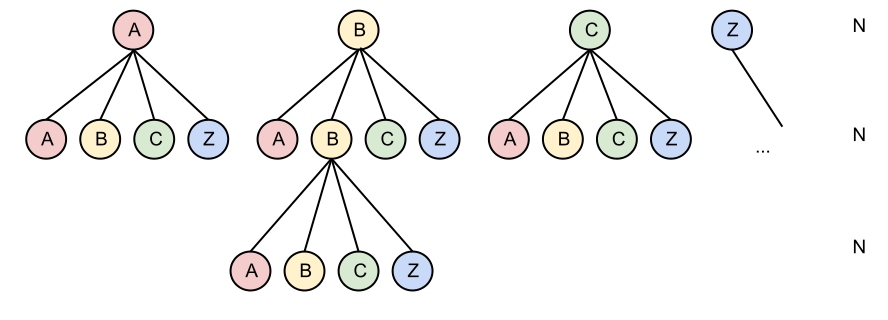
\includegraphics[width=10cm]{permutations_diag1}
\end{center}
Imagine having N marbles in a bag.  You draw a marble out, then put it back.  The first time you draw there are \(n\) possibilities.  This becomes the first position in your permutation. You have \(n\) different permutations\\
\\
The next time your draw, you have \(n\) possibilities again.  For each of the previous \(n\), they have \(n\) possiblities for the second position.  Now you have \(n\times n = n^2\). \\
\\
This will continue until you have drawn m times
\\
Therefore
\[{n\choose m} = n^m\]


\section{ Permutation: n Choose m with No Replacement}
The equation for n objects taken m at a time without replacement is
\[{n\choose m} = \frac{n!}{(n-m)!}\]
This is read as "n choose m" without replacement\\
\\
\subsection{Conjecture}
\begin{center}
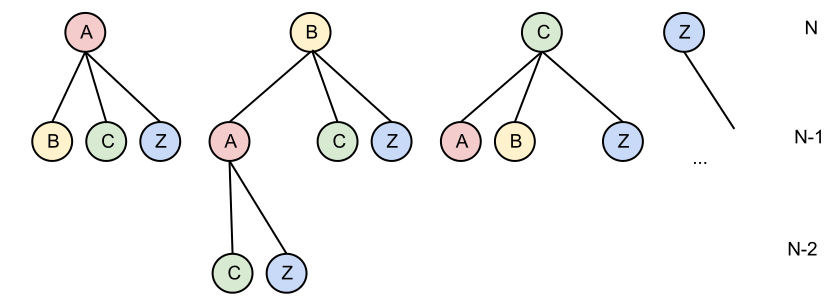
\includegraphics[width=10cm]{permutations_diag2}
\end{center}
Imagine having N marbles in a bag.  You draw a marble out, but do not put it back in the bag.  The first time you draw there are \(n\) possibilities.  This becomes the first position in your permutation. You have \(n\) different permutations\\
\\
The next time your draw, you have only \(n-1\).  For each of the previous \(n\), they have \(n\) possiblities for the second position.  Now you have \(n\times (n-1)\). \\
\\
The next time your draw, you have \(n-2\).  For each of the previous \(n-1\), they have \(n-2\) possiblities for the third position.  Now you have \(n\times (n-1) \times (n-2) \). \\
If this continued until there were no marbles left, you would have \(n(n-1)(n-2)...(2)(1) = n!\), but you stop after \(m\) times ( where \(m<n\)).  This can be written as:\\
\begin{align*}
{n \choose m} &= \frac{n(n-1)(n-2)...(n-m)(n-m-1)...(2)(1)}{(n-m)(n-m-1)...(2)(1)}\\
{n \choose m} &= \frac{n!}{(n-m)!}
\end{align*}
\\
\section{ Combination: n Choose m with Replacement}
\[{n \choose m} = \frac{n^m}{m!}\]

\subsection{Conjecture}
A Combination is the same as a permutation, but where order is not important.  So ABC, BAC, CBA, and so forth, are all the same.\\
\\
So start with the the equation for permuation with replacement, then we will reduce it by the number of the number of permuations in the sequence. So\\
\[{n \choose m} = n^m\]
With \(m!\) being unique, so\\
\[{n \choose m} = \frac{n^m}{m!}\]

\section{ Combination: n Choose m with No Replacement}
\[{n \choose m} = \frac{n!}{m!(n-m)!}\]

\subsection{Conjecture}
A Combination is the same as a permutation, but where order is not important.  So ABC, BAC, CBA, and so forth, are all the same.\\
\\
So start with the the equation for permuation without replacement, then we will reduce it by the number of the number of permuations in the sequence. So\\
\[{n \choose m} = \frac{n!}{(n-m)!}\]
With \(m!\) being unique, so\\
\[{n \choose m} = \frac{n!}{m!(n-m)!}\]

\chapter{Differential Calculus}

\section{Chain Rule}

\section{Product Rule}
The Product Rule is most commonly stated as
\[(f(x)g(x))' = f'(x)g(x) + f(x)g'(x)\]
or more formally as
\[\frac{d}{dx}\bigg[f(x)g(x) \bigg] = \frac{df}{dx}g(x) + f(x)\frac{dg}{dx} \]

\subsection{Derivation}
Using
\[\frac{df}{dx} = \lim_{h\to0}\frac{f(x+h) -f(x)}{h} \text{, the Formal Definition of the Derivative}\]
\begin{align*}
\frac{d}{dx}\bigg[f(x)g(x) \bigg] =& \lim_{h\to0}\frac{f(x+h)g(x+h) -f(x)g(x)}{h} \\
=& \lim_{h\to0}\frac{f(x+h)g(x+h) + [f(x+h)g(x) - f(x+h)g(x)] - f(x)g(x)}{h} \\
=& \lim_{h\to0}\frac{f(x+h)g(x+h) - f(x+h)g(x) + f(x+h)g(x) - f(x)g(x)}{h} \\
=& \lim_{h\to0}\frac{f(x+h)g(x) - f(x)g(x)}{h} + \lim_{h\to0}\frac{f(x+h)g(x+h) - f(x+h)g(x)}{h} \\
=& \lim_{h\to0}\bigg(\frac{f(x+h) - f(x)}{h}g(x)\bigg) + \lim_{h\to0}\bigg(f(x+h)\frac{g(x+h) - g(x)}{h}\bigg) \\
=& \lim_{h\to0}\frac{f(x+h) - f(x)}{h}\lim_{h\to0}g(x) + \lim_{h\to0}f(x+h)\lim_{h\to0}\frac{g(x+h) - g(x)}{h} \\
=& \bigg(\lim_{h\to0}\frac{f(x+h) - f(x)}{h}\bigg)g(x) + f(x)\bigg(\lim_{h\to0}\frac{g(x+h) - g(x)}{h}\bigg) \\
\frac{d}{dx}\bigg[f(x)g(x) \bigg] =& \frac{df}{dx}g(x) + f(x)\frac{dg}{dx}
\end{align*}

\section{Derivative of a Polynomial}
\[ \frac{d}{dx}\bigg[\sum\limits_{n=0}^N{a_n x^n} \bigg] = \sum\limits_{n=0}^N{a_n n x^{n-1}}\]

\subsection{Derivation}
\[\frac{df}{dx} = \lim_{h\to0}\frac{f(x+h) -f(x)}{h} \text{, the Formal Definition of the Derivative}\]
\[f(x) = \sum\limits_{n=0}^N{a_n x^n}\]
\begin{align*}
\frac{df}{dx} =&  \lim_{h\to0}\frac{\sum\limits_{n=0}^N{a_n (x+h)^n} - \sum\limits_{n=0}^N{a_n x^n}}{h} \\
=&  \lim_{h\to0}\frac{\sum\limits_{n=0}^N{a_n \sum\limits_{i=0}^n{{n \choose i}x^{n-i}h^i}} - \sum\limits_{n=0}^N{a_n x^n}}{h} \\
=&  \lim_{h\to0}\frac{
\sum\limits_{n=N}^0{a_n [{n\choose0}x^n + {n\choose1}x^{n-1}h+ {n\choose1}x^{n-2}h^2 + ... + {n\choose n}h^n]} - \sum\limits_{n=N}^0{a_n x^n}}
{h} \\
=&  \lim_{h\to0}\frac{\sum\limits_{n=N}^0{a_n x^n} + \sum\limits_{n=N}^0{{n\choose1} a_n x^{n-1}h} + \sum\limits_{n=N}^0{{n\choose1} a_n x^{n-2}h^2 + ... + \sum\limits_{n=N}^0{{n\choose n} a_n h^n}} - \sum\limits_{n=N}^0{a_n x^n}}{h} \\
=&  \lim_{h\to0} \frac{ 
\sum\limits_{n=N}^0{ {n\choose1} a_n x^{n-1}h   } + 
\sum\limits_{n=N}^0{ {n\choose1} a_n x^{n-2}h^2 } + ... + 
\sum\limits_{n=N}^0{ {n\choose n}a_n      h^n}  }{h} \\
=& \sum\limits_{n=N}^0{ {n\choose1} a_n x^{n-1}  }\\
\frac{df}{dx} =& \sum\limits_{n=N}^0{ a_n n x^{n-1}  }\\
\end{align*}

\section{Derivative of Sine}
\section{Derivative of Cosine}

\section{Derivative of $e^x$}
\[ \frac{d}{dx}\bigg[e^x \bigg] = e^2 \]

\subsection{Derivation}
\[\frac{df}{dx} = \lim_{h\to0}\frac{f(x+h) -f(x)}{h}  \text{, the Formal Definition of the Derivative} \]
\[ f(x) = e^x \]
\begin{align*}
\frac{df}{dx} =& \lim_{h\to0}\frac{e^{(x+h)} - e^x}{h} \\
=& \lim_{h\to0} e^x\frac{(e^h - 1)}{h} \\
=& e^x \lim_{h\to0} \frac{(e^h - 1)}{h}
\end{align*}
Let \( u = e^h -1 \) , so \(\ln{(u+1)} = h \) \\
and when \( h\to 0 \) , also  \(u \to 0\)
\begin{align*}
\frac{df}{dx} =& e^x \lim_{h\to0} \frac{u}{\ln{(u+1)}} \\
=& e^x \lim_{h\to0} \frac{1}{\frac{1}{u}\ln{(u+1)}} \\
=& e^x \lim_{h\to0} \frac{1}{\ln{\left((u+1)^{\frac{1}{u}}\right)}} \\
=& e^x  \frac{1}{\ln{\left(\lim_{h\to0}(u+1)^{\frac{1}{u}}\right)}} \\
\end{align*}
Recall the definition of \(e\)
\[\lim_{n\to0}(n+1)^{\frac{1}{n}}\]\\
So
\begin{align*}
\frac{df}{dx} =& e^x  \frac{1}{\ln{\left(\lim_{h\to0}(u+1)^{\frac{1}{u}}\right)}} \\
 =& e^x  \frac{1}{\ln{(e)}} \\
 \frac{df}{dx} =& e^x
\end{align*}

\section{Derivative of $\ln(x)$}
\[ \frac{d}{dx}\bigg[\ln(x) \bigg] = \frac{1}{x} \]

\subsection{Derivation}
\[\frac{df}{dx} = \lim_{h\to0}\frac{f(x+h) -f(x)}{h}  \text{, the Formal Definition of the Derivative} \]
\[ f(x) = \ln{(x)} \]
\begin{align*}
\frac{df}{dx} =& \lim_{h\to0}\frac{\ln{(x+h)} - \ln(x)}{h} \\
=& \lim_{h\to0}\frac{ \ln{\left(\frac{x+h}{x}\right)} }{h} \\
=& \lim_{h\to0}\frac{1}{h} \ln{\left(1+ \frac{h}{x}\right)} \\
\end{align*}
Let \(u = \frac{h}{x}\), \\
And \(h = ux \) \\
\begin{align*}
\frac{df}{dx} =& \lim_{h\to0} \ln{\left(1+ u\right)^\frac{1}{ux}} \\
=& \lim_{h\to0} \frac{1}{x}\ln{\left((1+ u)^\frac{1}{u}\right)} \\
=&  \frac{1}{x}\lim_{h\to0}\ln{\left((1+ u)^\frac{1}{u}\right)} \\
=&  \frac{1}{x}\ln{\left(\lim_{h\to0}(1+ u)^\frac{1}{u}\right)} \\
\end{align*}
Recall the definition of \(e\)
\[\lim_{n\to0}(n+1)^{\frac{1}{n}}\]\\
So
\begin{align*}
\frac{df}{dx} =& \frac{1}{x}\ln{\left(\lim_{h\to0}(1+ u)^\frac{1}{u}\right)} \\
=& \frac{1}{x}\ln{(e)} \\
\frac{df}{dx} =& \frac{1}{x}
\end{align*}

\section{Derivative of $x^x$}
\[ \frac{d}{dx}\bigg[x^x \bigg] = x^x(\ln{(x)} + 1) \]

\subsection{Derivation}
Instead of deriving this from the Formal Definition of the Limit, we will use the previous derivatives as axioms with which to derive this one.
\begin{align*}
f(x)  =& x^x \\
\ln{(f(x))} =& \ln{(x^x)} \\
\ln{(f(x))} =& x\ln{(x)} \\
\frac{d}{dx}\bigg[\ln{(f(x))}\bigg] =& \frac{d}{dx} \bigg[ x\ln{(x)} \bigg] = \frac{d}{dx}\bigg[ x \bigg]\ln{(x)} + x\frac{d}{dx}\bigg[\ln{(x)} \bigg]\\
\frac{1}{f(x)}\frac{df}{dx} =&  \ln{(x)} + x\frac{1}{x} \\
\frac{df}{dx} =&  x^x(\ln{(x)} + 1)
\end{align*}

\chapter{Integral Calculus}

\section{Integration by Parts}
Integration by parts is most commonly stated as
\[\int{udv} = uv - \int{vdu}\]
Where both the functions u and v are implied to be functions of another variable, u(x) and v(x)

\subsection{Derivation}
Integration by parts can be derived starting with the Product Rule
\begin{align*}
d\left[ u(x)v(x) \right] &= \frac{du}{dx}v(x) + u(x)\frac{dv}{dx} \\
\int{d\left[ u(x)v(x) \right]dx} &= \int{\left(\frac{du}{dx}v(x) + u(x)\frac{dv}{dx}\right)dx} \\
u(x)v(x) &= \int{\frac{du}{dx}v(x)dx} + \int{u(x)\frac{dv}{dx}dx} \\
u(x)v(x) - \int{\frac{du}{dx}v(x)dx} &=  \int{u(x)\frac{dv}{dx}dx} \\
\int{u(x)dv} &= u(x)v(x) - \int{v(x)du} \\
\end{align*}
Or more informally written as
\begin{align*}
\int{udv} &= uv - \int{vdu} 
\end{align*}

\chapter{Vector Calculus}
\section{Vector Dot Product}
\section{Vector Cross Product}
\section{Curl of a Gradient}
\section{Curl of the Curl}
\section{Divergence of a Gradient}
\section{Divergence of the Curl}

\chapter{Statistics}

\chapter{Probability}
\section{Baye's Theorem}

\chapter{Discrete Mathematics}

\section{Amitorization Formula}
The formula to calculate equal payments \(p\) to reduce an initial debt \(d\) in \(N\) payments with interest rate \(r\) is\\

\[p = d\frac{r(1+r)^N}{(1+r)^N -1}\]

\subsection{Derivation}
\(y(n)\) is the balance on the loan at compound iteration \(n\), where \(n \in \mathbb{I} \)\\
\(y(0) = d\) \\
Each compounding period, a payment of \(p\) will be made.\\
Each compounding period, an interest rate of \(r\) will be applied to the balance.
\(N\) will be the total number of payments.\\

\begin{align*}
y(0) &= d \\
y(1) &= y(0) + y(0)r - p = (1+r)y(0) -p\\
y(2) &= (1+r)y(1) -p = (1+r)((1+r)d -p) -p \\
y(3) &= (1+r)y(2) -p = (1+r)((1+r)((1+r)d -p) -p) -p \\
y(n) &= d(1+r)^n -p(1+r)^{n-1} -p(1+r)^{n-2} -p(1+r)^{n-3} - ...\\
\\
y(n) &= d(1+r)^n -p\sum\limits_{i=0}^{n-1}{{(1+r)}^i}
\end{align*}
This formula tells us the balance at any given compounding period.  What would the payment, \(p\), have to be in order for balance to be 0 when \(n=N\)?\\
\begin{align*}
y(N) &= d(1+r)^N -p\sum\limits_{i=0}^{N-1}{{(1+r)}^i} \\
0 &= d(1+r)^N -p\left( \frac{1-(1+r)^N}{1-(1+r)} \right) \\
p\left( \frac{(1+r)^N -1}{r} \right) &= d(1+r)^N \\
p &= d\frac{r(1+r)^N}{(1+r)^N -1}
\end{align*}

\chapter{Other Stuff}

\section{Euler's Formula}
Euler's formula is most commonly written as 
\[e^{i\theta} = \cos{\theta} + i\sin{\theta}\]

\subsection{Derivation}
Do a Taylor Series expansion on \(e^{i\theta}\)
\begin{align*}
f(x) &= \sum_{n=0}^{\infty}{\left.\dfrac{d^{(n)}}{dx}\bigg[f(x)\bigg]\right|_{x=x_0}\frac{(x-x_0)^n}{n!}} \\
e^{i\theta} &= \sum_{n=0}^{\infty}{\left.\dfrac{d^{(n)}}{d\theta}\bigg[f(\theta)\bigg]\right|_{\theta=0}\frac{(\theta)^n}{n!}} \\
e^{i\theta} &= e^{i0}\frac{\theta^0}{0!} + e^{i0}i\frac{\theta^1}{1!} +e^{i0}i^2\frac{\theta^2}{2!}+e^{i0}i^3\frac{\theta^3}{3!}+e^{i0}i^4\frac{\theta^4}{4!}+e^{i0}i^5\frac{\theta^5}{5!}+e^{i0}i^6\frac{\theta^6}{6!}... \\
e^{i\theta} &= 1 + i\frac{\theta}{1!} - \frac{\theta^2}{2!}-i\frac{\theta^3}{3!}+\frac{\theta^4}{4!}+i\frac{\theta^5}{5!}-\frac{\theta^6}{6!}+... \\
e^{i\theta} &= 1 - \frac{\theta^2}{2!}+\frac{\theta^4}{4!}-\frac{\theta^6}{6!} + ... + i\frac{\theta}{1!}-i\frac{\theta^3}{3!}+i\frac{\theta^5}{5!} + ... \\
e^{i\theta} &= \underbrace{\bigg(1 - \frac{\theta^2}{2!}+\frac{\theta^4}{4!}-\frac{\theta^6}{6!} + ...\bigg)}_{cos\theta} + i\underbrace{\bigg(\frac{\theta}{1!}-\frac{\theta^3}{3!}+\frac{\theta^5}{5!} + ...\bigg)}_{sin\theta} \\
e^{i\theta} &= \cos{\theta} + i\sin{\theta}
\end{align*}

\chapter*{Acknowledgements}

\section*{Credits}

\end{document}